\subsection{Функция источника}
\label{sec:source_section}
Спектр рентгеновской трубки является характеристическим, спектральная часть
 которого достаточно хорошо описывается двумя функциями Лоренца взятыми с
 весовыми коэффициентами (\ref{eq:source_spectral}).

 \begin{equation} \label{eq:source_spectral}
   g_{\lambda} (\lambda) = \frac{2\pi}{3}  \left \{ \frac{\delta\lambda_1}{(\lambda - \lambda_1)^2+
   (\delta \lambda_1)^2} + \frac{1}{2} \frac{\delta\lambda_2}{(\lambda-\lambda_1)^2+(\delta\lambda_1)^2} \right \}
  \end{equation}

  Плотность распределения количества потока электромагнитного излучения в зависимости от угла
  отстройки относительно прямолинейного распределения задается функцией Гаусса \ref{eq:source_angle}.

  \begin{equation} \label{eq:source_angle}
    g_{\vartheta} (\vartheta) = \frac{1}{\sigma \sqrt{ 2\pi}} exp  ( -\frac{\vartheta^2}{2\sigma^2} )
   \end{equation}
где $\sigma$ - параметр, который характеризует ширину углового распределения на половине высоты.

\begin{figure}[H]
  \centering
  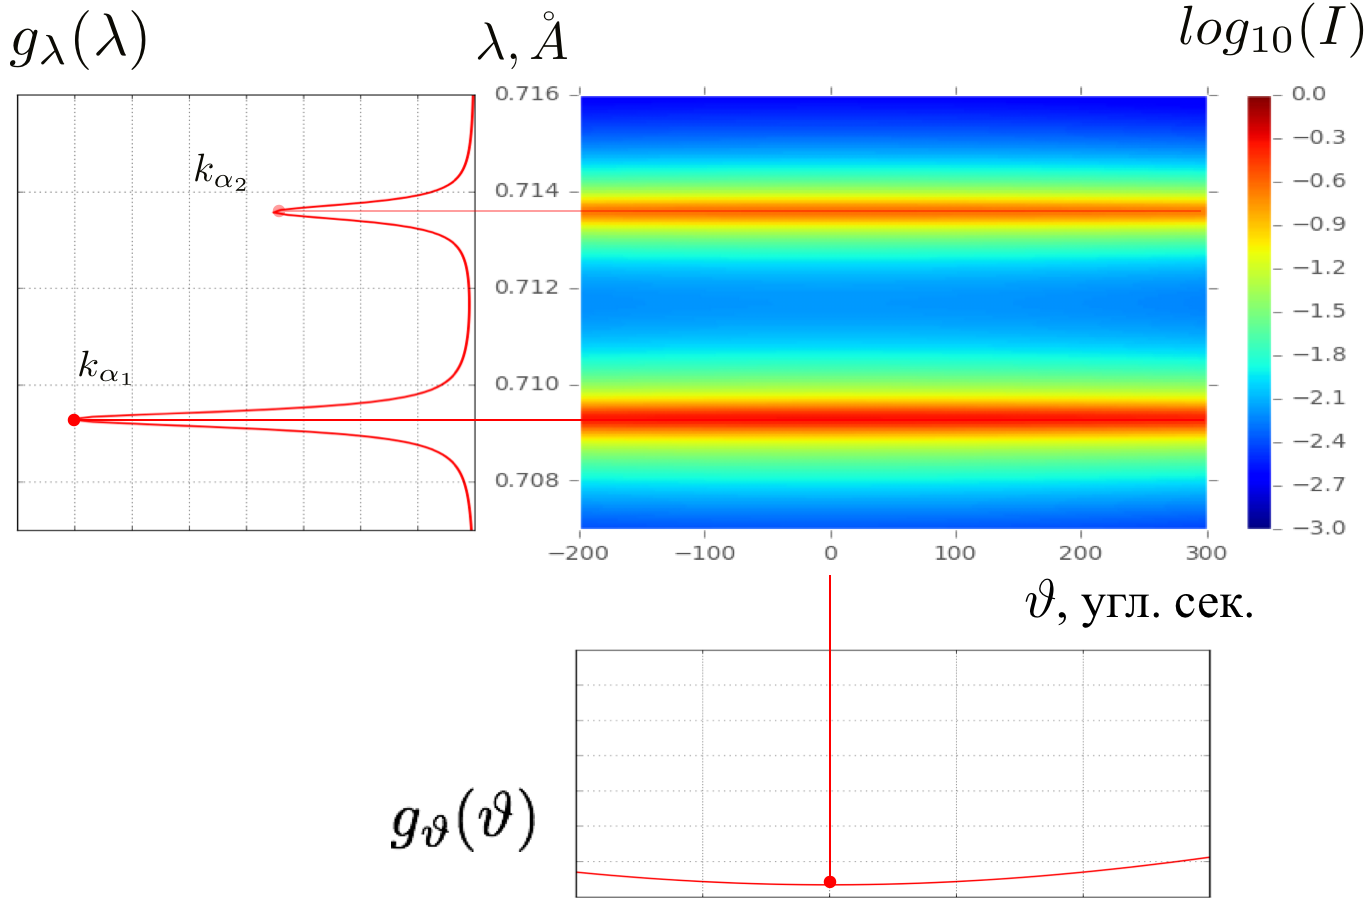
\includegraphics[width=0.6\textwidth]{images/source_distrubition.png}
  \caption{Спектрально – угловое распределение лабораторного источника рентгеновского
   излучения с молибденовым анодом, угловая полуширина распределения составляет $\sigma = 600$ угл. сек. }
  \label{ris:source_distrubition}
\end{figure}


 \subsection{Функция щелевых коллиматоров}
 \label{sec:slits_section}
 Рассмотрим преобразование пучка рентгеновского излучения проходящего через систему щелевых коллиматоров.
 \begin{figure}[H]
   \centering
   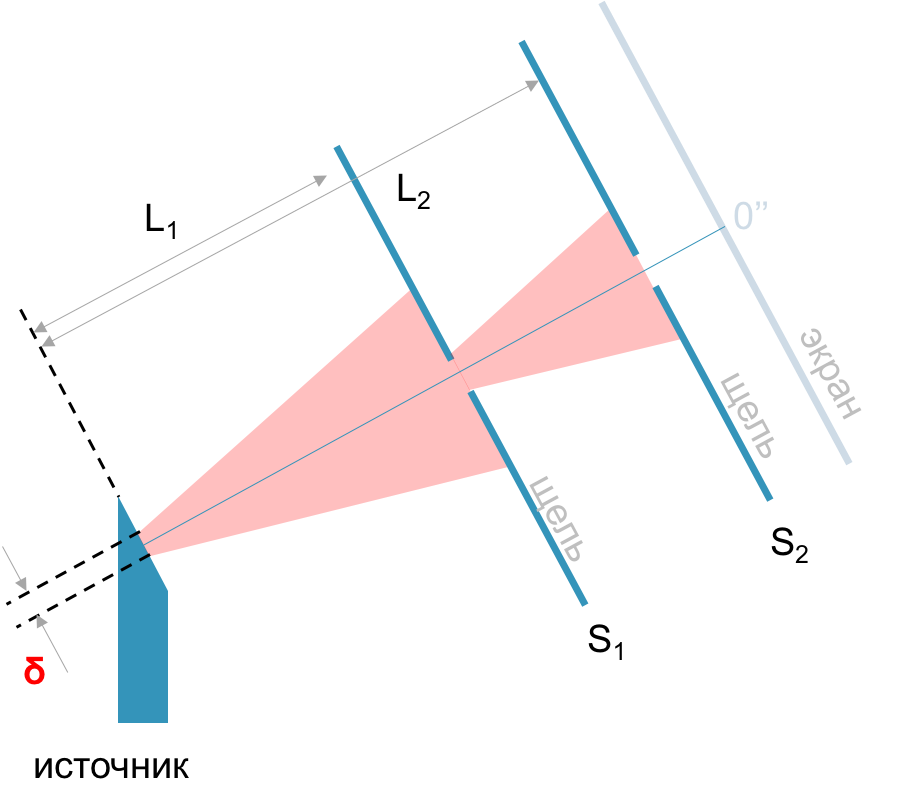
\includegraphics[width=0.6\textwidth]{images/for_slits.png}
   \caption{Схематичное представление щелевых устройств}
   \label{ris:for_slits}
 \end{figure}

На начальном этапе мы рассматривали модель точечного источника излучения $\delta = 0$.
В таком случае, интенсивность проходящего излучения будет определятся
одним щелевым устройством, которое является более узким в пересчете в угловые
координаты. Например, для фиксированных расстояний между элементами,
($L_1 = 570$ мм, $L_2 = 1005$ мм), в случае одинаковых линейных размеров щелей и точечного
источника, интенсивность будет определяться более удаленным щелевым устройством и
распределение интенсивности принимает вид ступеньки (рисунок ~\ref{ris:sourc_map_a}). Если источник является
 продолжительным $\delta \neq 0$, то угловое распределение интенсивности принимает более сложный вид, как показано на рисунке ~\ref{ris:sourc_map_b}.



 \begin{figure}[H]
   \centering
   \subfloat[Точечный источник]{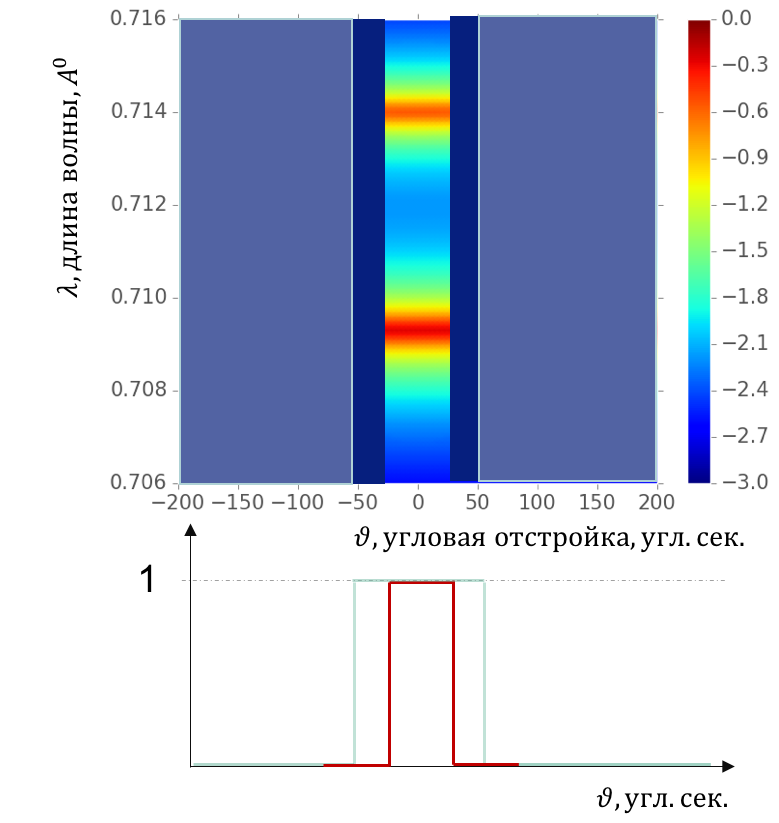
\includegraphics[width=0.5\textwidth]{images/point_sourc_map.png}\label{ris:sourc_map_a}}
   \hfill
   \subfloat[Источник с линейным размером $\delta = 0.2$ мм]{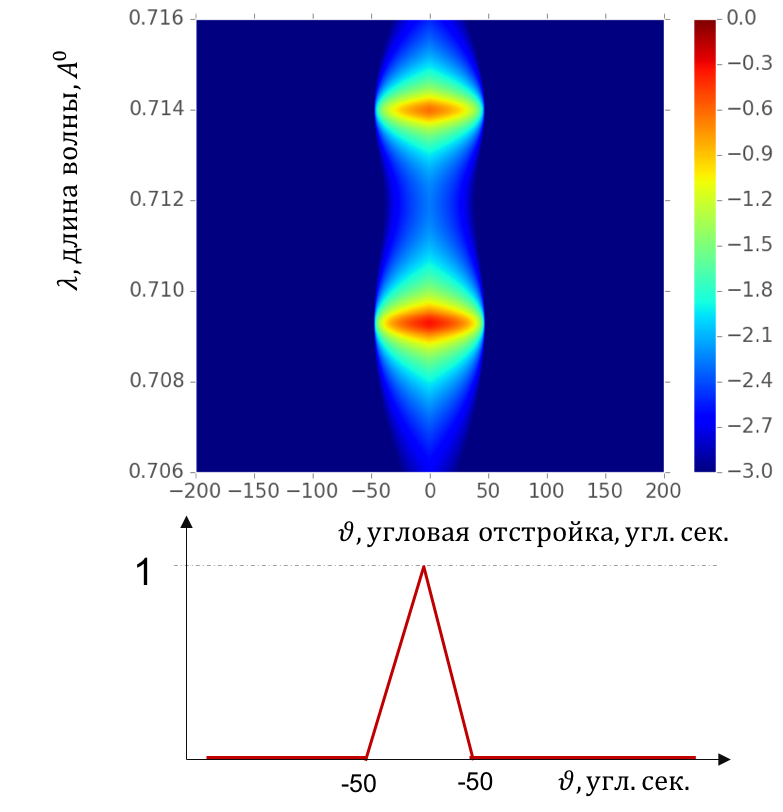
\includegraphics[width=0.5\textwidth]{images/wide_sourc_map.png}\label{ris:sourc_map_b}}
   \caption{Спектрально угловое распределение источника в система двух щелей}
   \label{ris:sourc_map}
 \end{figure}

 Необходимо отметить, что для описания дифракционного эксперимента важно расчитывать именно
 угловое распределение, т.е. знать количество и величину энергии квантов падающих под тем
 или иным углом на кристалл. Для того, чтобы это сделать нам необходимо посчитать площадь параллелограммов
 (рисунок \ref{ris:how_many_quants_use_parallelogr}),

 \begin{figure}[H]
   \centering
   \subfloat[Пропускная способность системы пропорциональна площади
   соответствующего параллелограмма ]{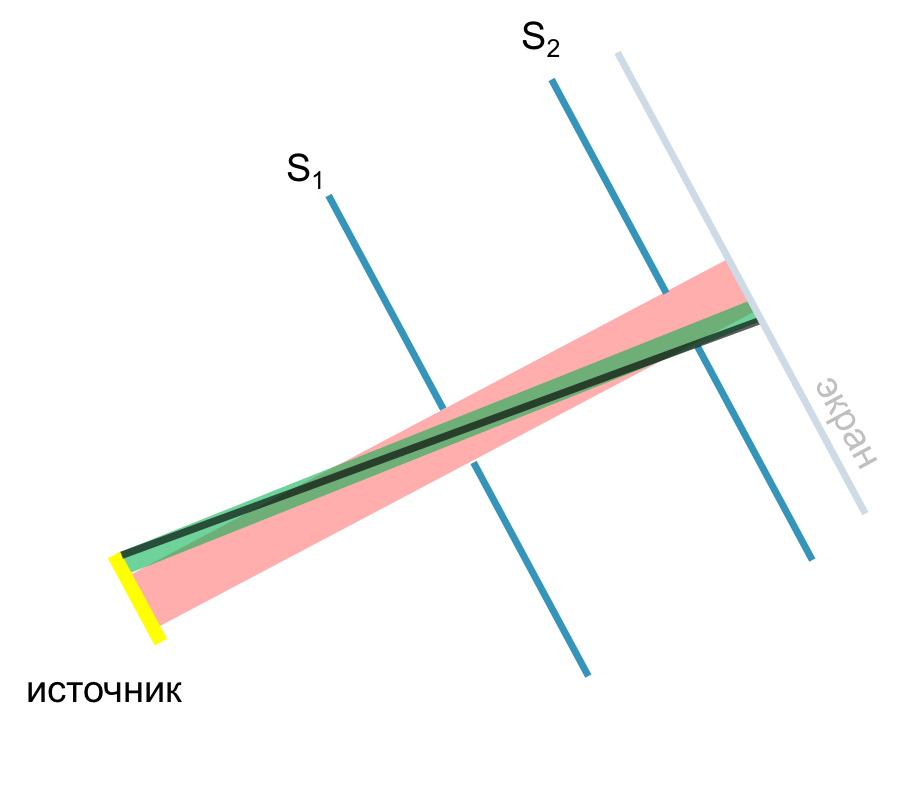
\includegraphics[width=0.45\textwidth]{images/how_many_quants_use_parallelogr_1.png}}
   \hfill
   \subfloat[Интенсивность на экране $\delta = 0.2$ мм,  \textcolor{mygreen}{Ось ординат $g_S(\vartheta)$}]{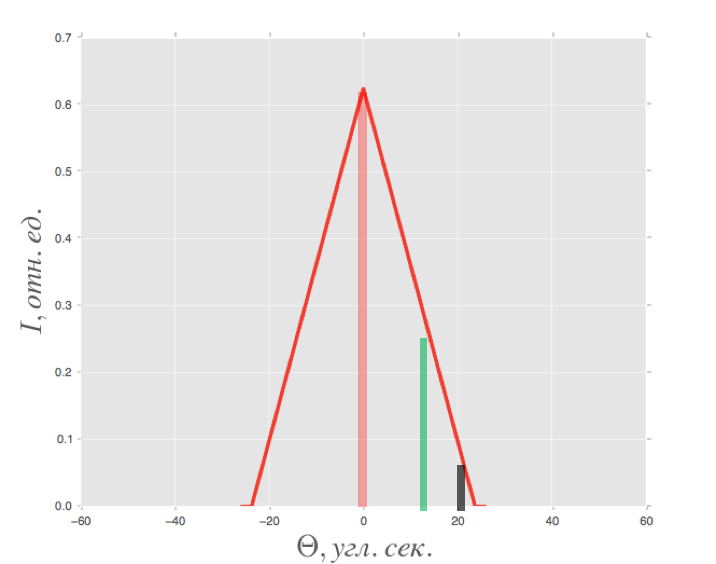
\includegraphics[width=0.45\textwidth]{images/how_many_quants_use_parallelogr_2.png}}
   \caption{Схематичное представление расчета интенсивности углового
   распределения излучения после прохождения системы щелевых коллиматоров}
   \label{ris:how_many_quants_use_parallelogr}
 \end{figure}
Более подробный расчет  $g_S(\vartheta)$ представлен в (\ref{sec:calc_slits_ability}).
На рисунке (\ref{ris:calc_slits_ability_res}) представлены результаты расчета пропускной способности системы двух щелей для некоторых параметров в
приближении точечного и продолжительного источника.

\begin{figure}[H]
  \centering
  \subfloat[$S_1 = S_2 = 50$ мкм; $\delta = 0.2$ мм;]{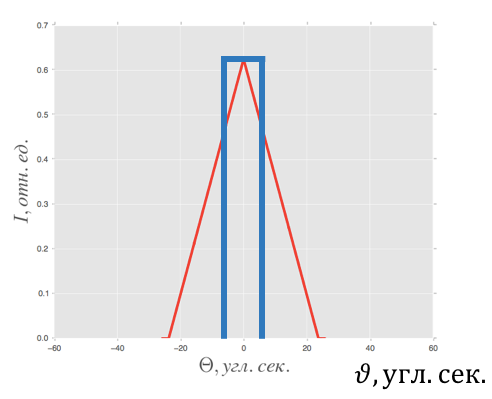
\includegraphics[height=6em]{images/calc_slits_ability_res_1.png}}
  \hfill
  \subfloat[$S_1 = 20$ мкм; $S_2 = 40$ мкм; $\delta = 0.2$ мм;]{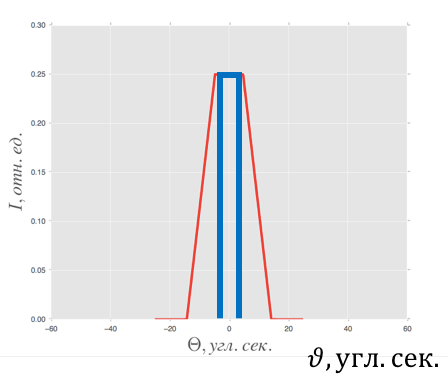
\includegraphics[height=6em]{images/calc_slits_ability_res_2.png}}
  \hfill
  \subfloat[$S_1 = 200$ мкм; $S_2 = 400$ мкм; $\delta = 0.2$ мм;]{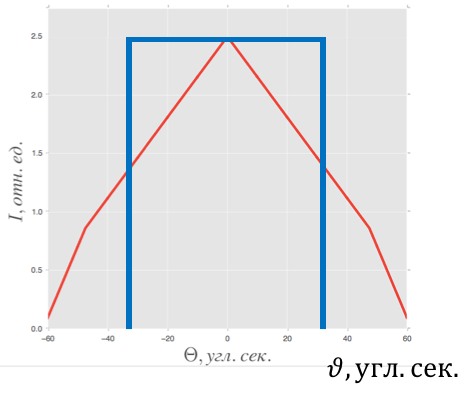
\includegraphics[height=6em]{images/calc_slits_ability_res_3.png}}
  \hfill
  \subfloat[$S_1 = 200$ мкм; $S_2 = 400$ мкм; $\delta = 0.1$ мм;]{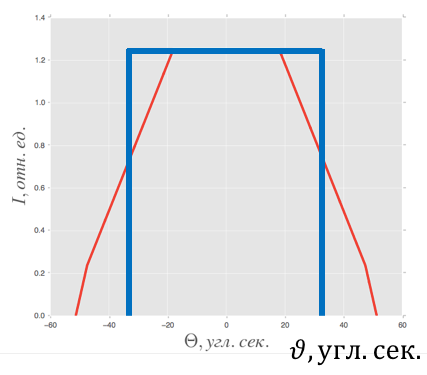
\includegraphics[height=6em]{images/calc_slits_ability_res_4.png}}
  \caption{$L_1 = 570$ мм; $L_2 = 1005 $ мм \textcolor{mygreen}{ Ось ординат $g_S(\vartheta)$}}
  \label{ris:calc_slits_ability_res}
\end{figure}

Анализ показывает что перегиб (рисунок \ref{ris:calc_slits_ability_res}) возникает вследствие переходного
процесса от точечного источника к бесконечному, т.е. на меньших углах плотность излучения определяется ближайшей
щелью к источнику, а после некоторого угла определяющей становится более удаленная \textcolor{mygreen}{НАРИСОВАТЬ РИСУНОК}(рисунок ).

\subsubsection{Дифракция на щели}
  Cowley1979ru на странице 47
